% !TEX root = ../../Article.tex
\chapter{Framework installation}
\label{app:D}
\section{Smart card development environment}
Setup guide for developing smart card applications using Eclipse 3.2.
\begin{enumerate}
  \item Unzip ``Smart\_card.zip''
  \item Install Java Development Kit 6u45. Use ``jdk-6u45-windows-i586.exe'' for 32-bit Windows. Other operating system versions can be found at: \sloppy \url{http://www.oracle.com/technetwork/java/javase/downloads/java-archive-downloads-javase6-419409.html#jdk-6u45-oth-JPR}
  \item Copy the contents of ``java\_card\_kit-2\_2\_2-windows'' to a directory of your choice.
  \item Copy the contents of ``eclipse-SDK-3.2.2-win32'' to a directory of your choice.
  \item Copy the contents from ``eclipse-jcde-0.2\\plugins'' into the plugin folder for Eclipse from previous step.
  \item Start Eclipse using the batch script ``RUN\_ME.bat''.
  \item In the toolbar select ``Java Card \textrightarrow Preferences'' and make sure the Java Card Development Kit path points to where the kit was installed. Refer to figure \ref{fig:javacardkit}.
  \item In the toolbar select ``JCWDE \textrightarrow Preferences'' and make sure the Java Card Development Kit path points to where the kit was installed. Refer to figure \ref{fig:javacardkit}.

\end{enumerate}

\begin{figure}[h!]
  \caption{Configuring Java Card kit 2.2.2 for Eclipse.}
  \label{fig:javacardkit}
  \centering
    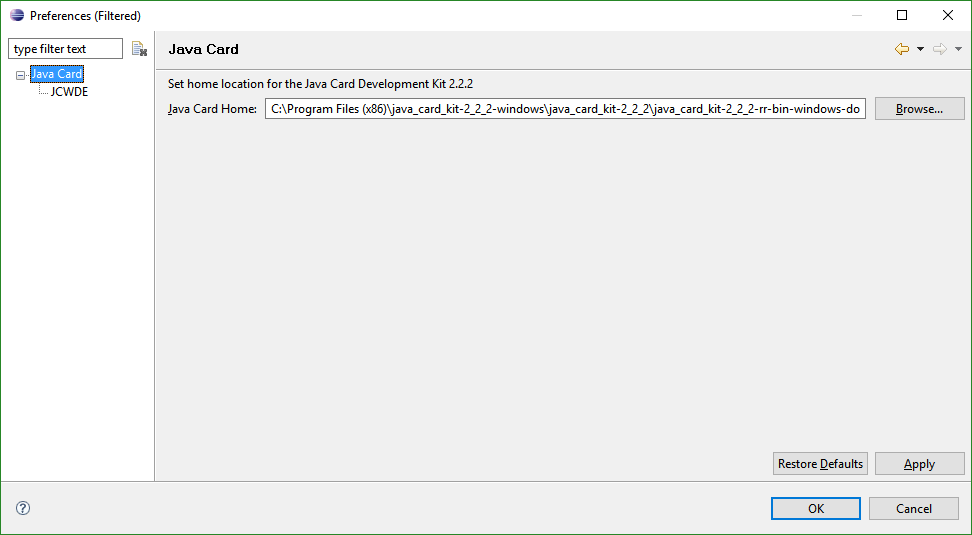
\includegraphics[width=0.95\textwidth]{images/eclipse_javacard.png}
\end{figure}

\section{Smart card deployment}
Setup guide for deploying smart card applications using GlobalPlatformPro (GP).
\begin{enumerate}
  \item Copy the contents of ``Smart\_card\_deployment'' to a directory of your choice.
  \item Configure ``runMe.bat'' and point to the correct .cap file.
  \item Run ``runMe.bat'' to delete and install your smart card application.
\end{enumerate}

\section{Smart card testing}
Setup guide for testing smart card applications using PyAPDUTool.
\begin{enumerate}
  \item Copy the contents of ``Smart\_card\_test\_tools'' to a directory of your choice.
  \item Run the tools.
\end{enumerate}

\section{Android development environment}
Setup guide for developing Android applications with our smart card library using Android Studio.
\begin{enumerate}
  \item Download the newest version of Android Studio from \sloppy \url{http://developer.android.com/sdk/index.html}
  \item Install Android SDK 6.0 using the Android SDK Manager.
  \item Add the libraries ``gPKIKeyStore'' and ``smartcardLibrary'' to your Android application. \sloppy \url{http://developer.android.com/sdk/installing/create-project.html#ReferencingLibraryModule}
  \item Fix any potential path issues.
\end{enumerate}
